\documentclass[12pt]{article}
\usepackage[utf8]{inputenc}
\usepackage{physics}
\title{Bachelorarbeit}
\author{Salem Rezik}
\date{September 2022}
\def\N{\bra{\Psi}\ket{\Psi}}
\def\muk{\overline{\mu}}
\usepackage{amsmath,amssymb}
\usepackage{graphicx}
\usepackage{wrapfig}
\usepackage{hyperref}
\usepackage[a4paper,left=1.3 in,right=1in,top=1in,bottom=1in]{geometry}
\usepackage[onehalfspacing]{setspace}

\begin{document}
\title{Semi-quantenmechanischer Variationsansatz zur Spindynamik in Quantenpunkten}
\maketitle
\tableofcontents

\newpage
\section{Motivation}
Die Realisierung von Quantencomputer mit genügend hoher Anzahl an Qubits wird oft als das „heilige Gral der Wissenschaft“ angesehen, denn 
es soll nach theoretischen Überlegungen, die über ein halbes Jahrhundert zurückführen, in der Lage sein, die Grenzen moderner Computer zu 
überschreiten. \\Im Gegensatz zum herkömmlichen Computer, der auf Basis von elektrischen Zuständen in Halbleitertransistoren funktioniert 
und nur die Zustände $\ket{0}$ oder $\ket{1}$ kennt, basiert der Quantencomputer auf quantenmechanische Zustände, wodurch u.a. eine 
drastisch höhere Anzahl von Zuständen auf gleichem Raum ermöglicht wird, was in bestimmten schnellere Prozesse.\\
Um sich dieses Problem zu verdeutlichen, wird der Hilbertraum eines N-Teilchen-Systems bestehend aus ½-Teilchen betrachtet, welches eine 
Dimension von $2^N$ besitzt; so dass allein die Speicherung aller Freiheitsgrade eines 100 Teilchen Systems eine unmögliche Herausforderung
 derzeitig ist. Dieses Problem hat schon damalige Physiker zu der Annahme verleitet, dass wohl ein theoretisch ein Computer basierend 
 auf quantenmechanischen Wirkungsmechanismen die wohl angebrachteste Lösung wäre. Und tatsächlich haben Bernstein and Vazirani 
 den ersten Beweis veröffentlicht, dass ein Quantencomputer in der Lage ist, das exponentielle Wachstum der Rechendauer auf ein 
 polynomiales Wachstum runterzubrechen.\\
Darüber hinaus können viele Algorithmen implementiert werden, dazu gehört auch der bekannte Shor-Algorithmus; ein Faktorisierungsverfahren,
welches unter anderem ein gewaltiges Sicherheitsrisiko für das übliche RSA-Kryptosystem darstellt.\\

\noindent Die zentralen Bausteine eines Quantencomputers sind die Quantencubits, kurz Qubits. Damit werden beliebige quantemechanische 
zwei-Niveau-Systeme sammelbezeichnet. In der Vergangenheit wurden bereits einige Realisierungsmöglichkeiten des Qubits umgesetzt.\\
Die Realisierungsvorschlag mit der sich diese Arbeit beschäftigt, ist die des Spins eines in einem Quantenpunkt eingefangenen 
Elektrons (Loch). Um diesen Spin zu beschreiben wird das Central-Spin-Model zur Beschreibung der Elektronepindynamik verwendet und mit 
dem semi-klassischen Variationsverfahren "Time-Dependent Variational Principle" (TDVP) behandelt.\\

\noindent Die Hoffnung liegt darin, durch Modifikationen von Parametern $\mu$ einer zu variierenden Wellen 
$\ket{\Psi} = \ket{\Psi(\mu_1,...,\mu_N)}$ das Problem des exponentiell zu N anwachsenden Hilbertraumes zu umgehen und gegenüber 
herkömmlichen, vollkommen quantenmechanischem Ansätzen mit größeren N möglichst kleine Abweichungen von der exakten Lösung zu erhalten.

\newpage






%%%%%%%%%%%%%%%%%%%%%%%%%% Quantenpunkte











\section{Quantenpunkte}
\noindent Diese Arbeit beschäftigt sich mit der mathematischen Modellierungen der Spindynamik eines Quantenpunktes, deshalb ist es 
sinnvoll vorab zu klären, was ein Quantenpunkt überhaupt ist. Damit einhergehend lassen sich die hier angenommenen Modelle begründen.\\



\begin{figure}[h!]
    \centering
    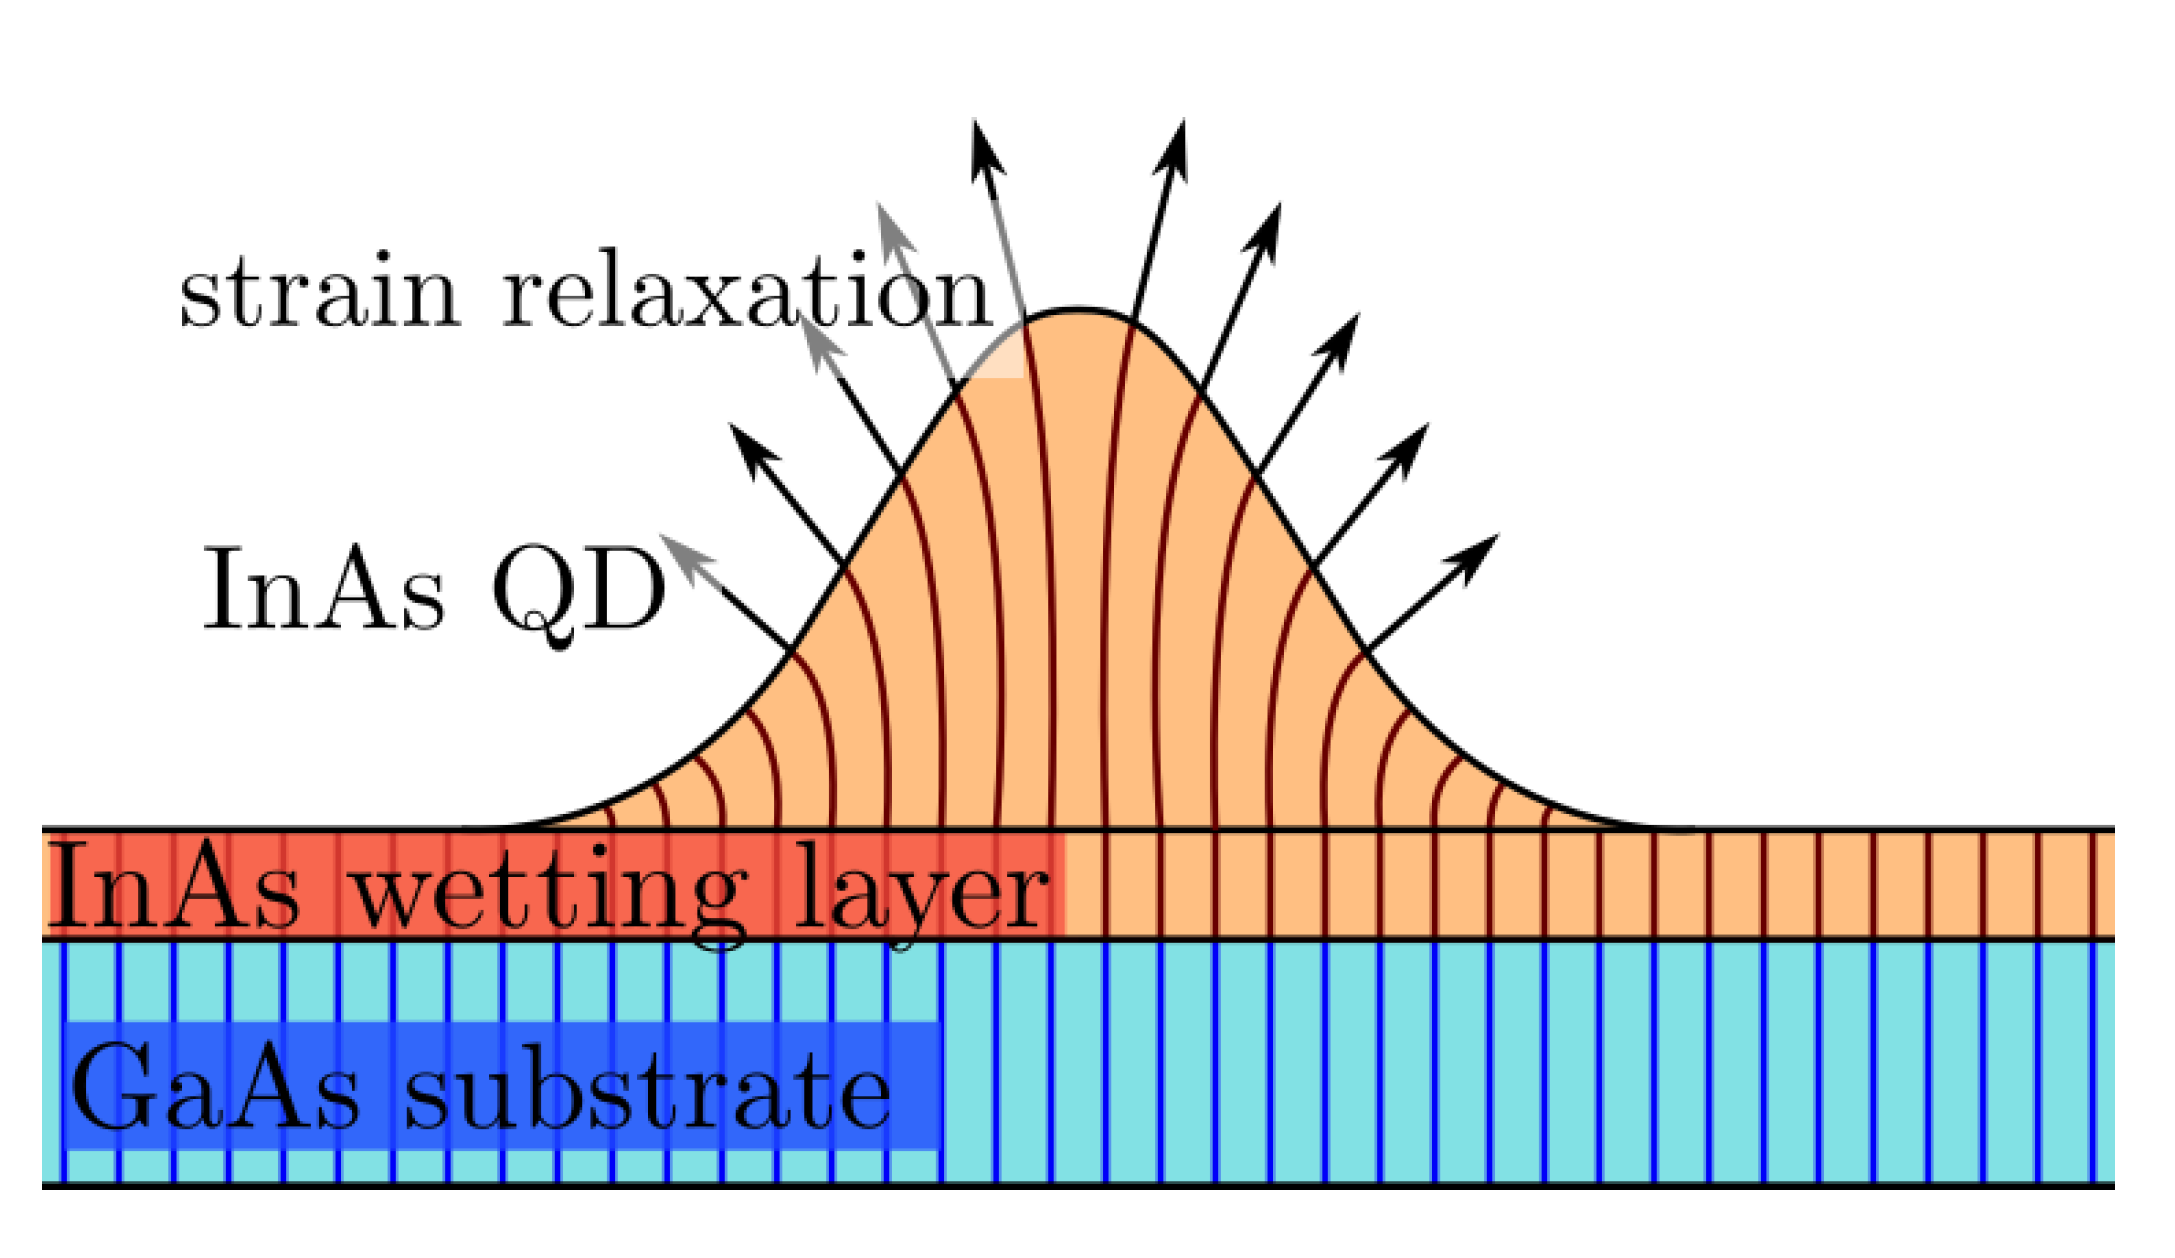
\includegraphics[width = 0.3\textwidth]{Abbildungen/QD_Schema.png}
    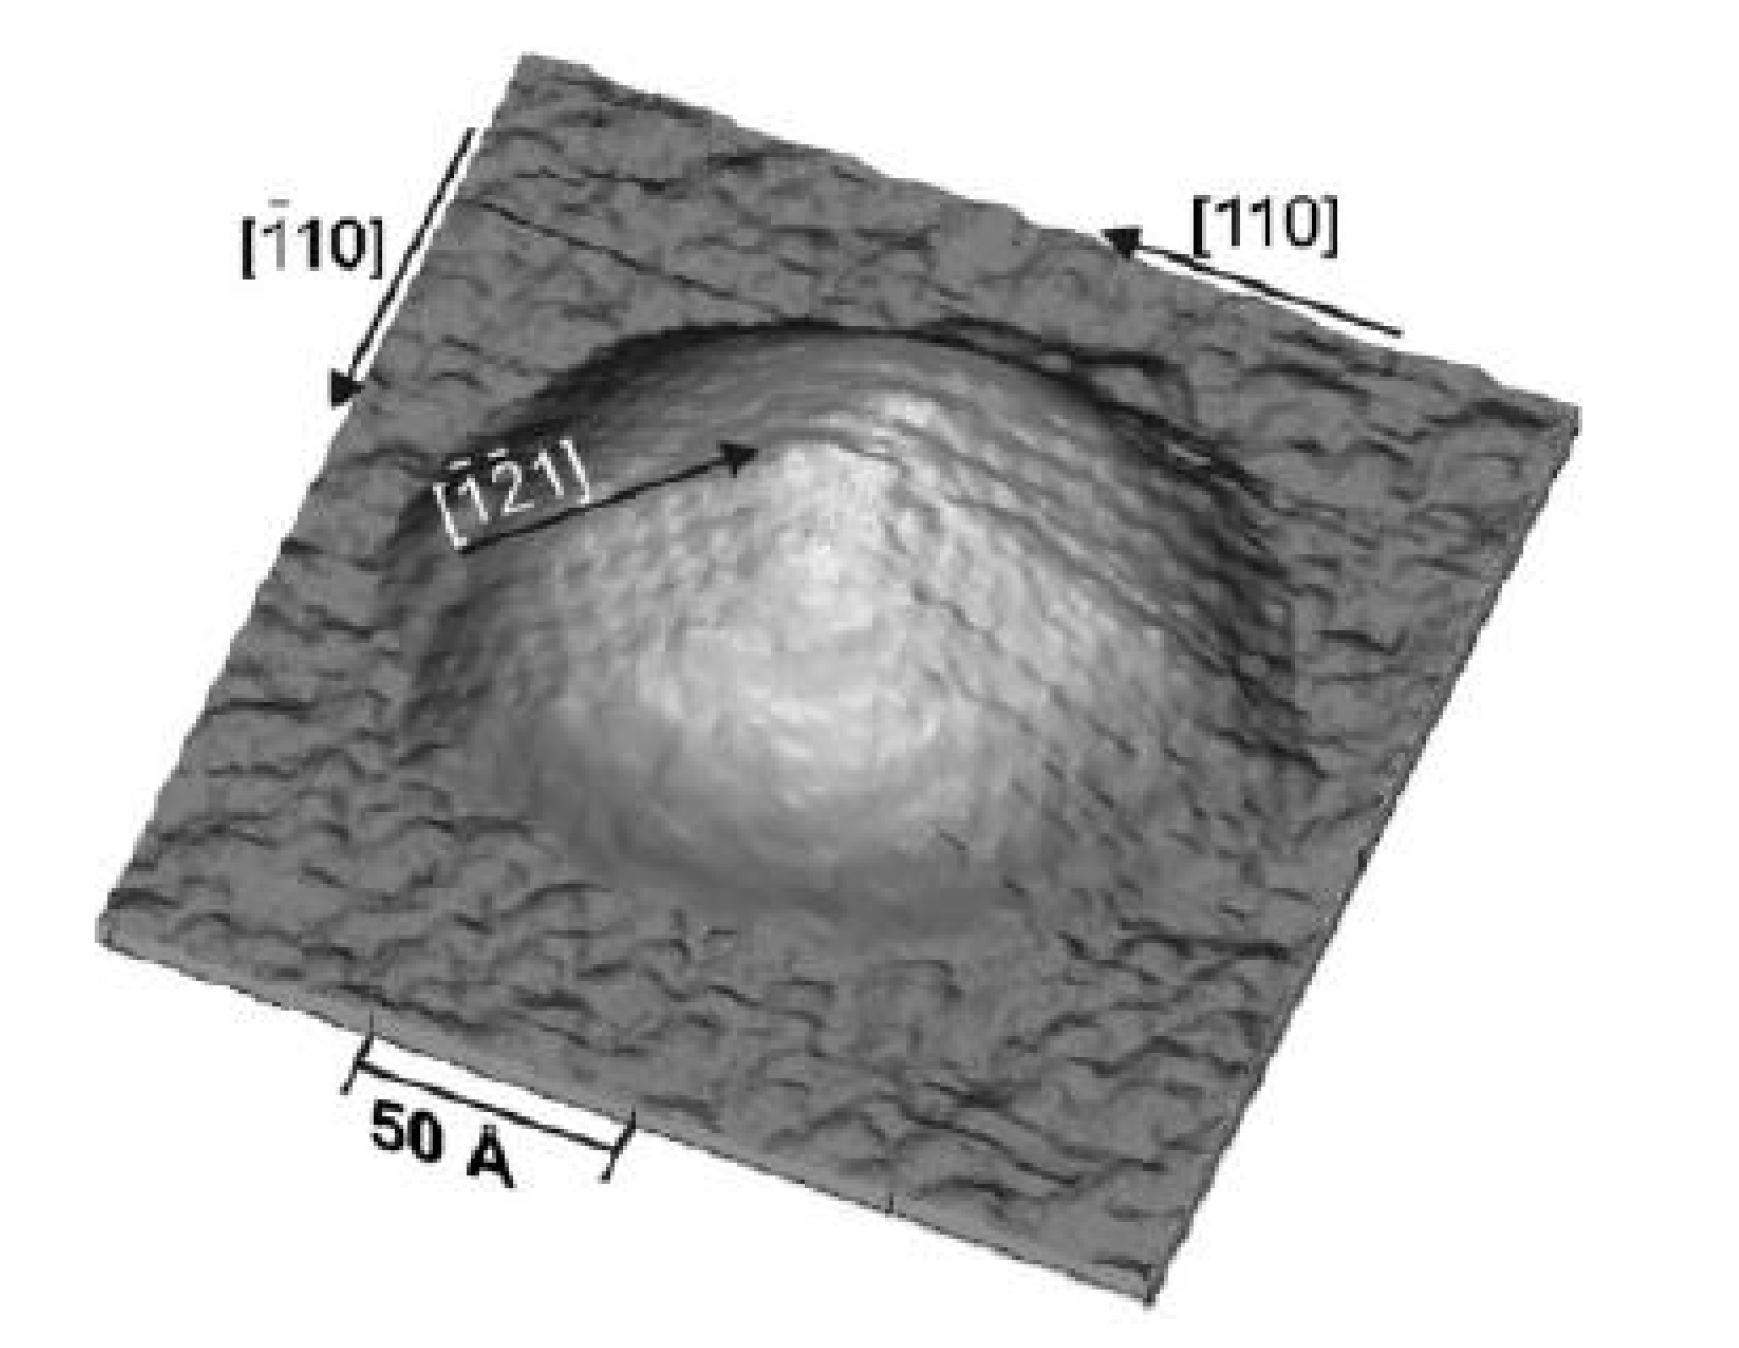
\includegraphics[width = 0.3\textwidth]{Abbildungen/einQD.png}
    \caption{Links:Schematischer Aufbau vom Wachstum eines InAs-Quantenpunkt auf einem GaAs-Substrat. Rechts: Automatisch 
    aufgelöstes Bild eines InAs-Quantenpunktes}
    \label{fig:QD_Schema}
\end{figure}

\noindent Die hier betrachten Quantenpunkte sind nanoskopische Halbleiterstrukturen, die wie ein dreidimensionaler Potentialtopf fungieren
 und einzelne Ladungsträger wie Elektronen oder Löcher einfangen können.\\
Die Stranski-Krastnov-Methode ist eine weitverbreitete Methode um Quantenpunkte zu erzeugen, dabei ist die Idee zwei Materialien mit 
unterschiedlicher Gitterkonstante mittels Molekularstrahlepitaxie aufeinander wachsen zu lassen. Der Kürze halber lässt es sich 
beispielhaft an den beiden Materialien InAs und GaAs erklären, denn dabei wird InAs-Schicht auf ein GaAs-Substrat wachsen gelassen, 
wobei die Gitterkonstante des InAs etwa 7\% größer ist, wodurch Spannung zwischen beiden Materialien entsteht. \\
\noindent Diese Spannung bewirkt Formationen von InAs-Inseln wie in \autoref{fig:QD_Schema} links zu sehen, die nur wenige zehn 
Nanometer groß sind, und verändert selbst die elektronische Eigenschaften, hauptsächlich den elektrische Feldgradienten des 
Quantenpunktes. Nun wird eine weiter Monoschicht GaAs auf das ganze Substrat gewachsen, so dass die InAs-Inseln vollständig von 
dem GaAs umschlossen sind. Diese umschlossenen InAs-Inseln bilden dann explizit den Quantenpunkt.\\


\begin{figure}
   \centering
    \includegraphics[width = 0.45\textwidth]{Abbildungen/QD_Energiebänder.png}
    \caption{Schematische räumliche Bandstruktur eines In(Ga)As/GaAs-Quantenpunktes mit den relevanten Bändern und einem 
    gefangenem Ladungsträger}
    \label{fig:QD_Bandstruktur}
\end{figure}
\noindent Das GaAs, welches den In(Ga)As Quantenpunkt umschließt, fungiert als Potentialtopf, denn die Energiebandlücke des InAs ist 
signifikant kleiner als die des GaAs. Nun kann ein einzelnes Elektron (Loch) räumlich einfangen werden und die Wechselwirkung mit dem 
Substrat unterdrückt werden, wodurch die Dekohärenzzeit deutlich verlängert werden kann. Eine kurze Dekohärenzzeit ist seit Beginn ein 
Hauptproblem bei der Realisierung des Quantencomputers. In \autoref{fig:QD_Bandstruktur} ist zu erkennen, dass einzelne Ladungsträger 
im InAs auf bestimmte Energieniveaus gefangen sind.\\
Dabei ist die Hyperfeinstruktur die dominante Wechselwirkung. Quantenpunkte werden deshalb auch als "künstliche Atome" bezeichnet,
 da ganz in Analogie zu Atomen ihre diskreten Enerigieniveaus von den eingefangen Teilchen besetzt werden können.









\newpage
\section{Time-Dependent Variational Principle }

Das grundlegende Prinzip der Time-Dependent Variatonal Principle, kurz TDVP, ist die Äquivalenz der zeitabhängigen Schrödingergleichung
 zu einem Extremisierungspropblem einer Wirkungsfunktion $S=\int_{t_1}^{t_2}L \thinspace dt$ mit der Lagrange-Funktion:

\begin{align}
    L\left(\overline{\Psi}(t), \Psi(t), t\right)=\frac{i}{2}\langle\Psi(t) \mid \dot{\Psi}(t)\rangle-\frac{i}{2}\langle\dot{\Psi}(t) \mid \Psi(t)\rangle-\langle\Psi(t)|\hat{H}(t)| \Psi(t)\rangle
\end{align}

Eine explizite Herleitung der Äquivalenz ist in (...) zu finden. \\

\noindent Für die Verwendung des Variationsverfahren ist es notwendig, dass der zu variierende Ansatz-Wellenfunktion 
$\ket{\Psi(\mu_1,...,\mu_N}$ analytisch ist. Da die Normierungsfunktion $N=N(\mu,\muk)$ nicht analytisch ist, wird sie 
für den modifizierten Ansatz ausgelassen. Da ein normierter Ansatz in diesem semi-klassischen Minimierungsverfahren nicht 
von Notwendigkeit ist, lassen sich folgende Bewegungsgleichungen hinschreiben:
\begin{align}
    i\dot{\mu_i} &= \sum_{j}\left(G_{ij}\right)^{-1}\thinspace \partial_{\overline{\mu_j}}\mathcal{H}
\end{align}

mit 
\begin{align}
    G_{ij} &= \frac{\bra{\partial_{\overline{\mu_i}}\Psi}\ket{\partial_{\mu_j}\Psi}}{\N} 
    - \frac{\bra{\partial_{\overline{\mu_i}}\Psi}\ket{\Psi}\bra{\Psi}\ket{\partial_{\mu_j}\Psi}}{\N^2} \\
    \mathcal{H} &= \frac{\bra{\Psi}\hat{H}\ket{\Psi}}{\N}
\end{align}

\noindent mit der Konvention: $\bra{\partial_{\overline{\mu_j}}\Psi} = \left(\thinspace\ket{\partial_{\mu_j}\Psi}\thinspace\right)^\dagger$

\noindent Mit dieser modifizierten Gram-Matrix $G_{ij}$ und dem modifizierten Hamiltonian $\mathcal{H}$, ist die Normierung wieder 
gesichert. 


\subsection{Wahl der Wellenfunktion}
\begin{wrapfigure}{r}{0.4\textwidth}
    \centering
    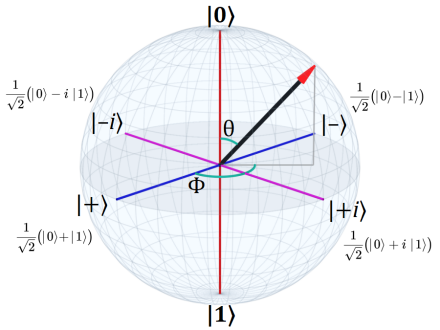
\includegraphics[width = 0.35\textwidth]{Abbildungen/bloch-sphere.png}
    \caption{Schematischer Aufbau einer Bloch-Sphere}
    \label{fig:qubit}
\end{wrapfigure}
Zur Vereinfachung werden alle Kernspin (wie der Elektronenspin) als 1/2-Spins angenähert. 
Die Wellenfunktion $\ket{\Psi}=\ket{\Psi(\mu_1(t),...,\mu_N(t)}$ enthält die zeitabhängigen Parameter $\mu_i(t)$ und realisiert einen 
kohärenten Zustand. Wir nutzen die Geometrie des 1/2-Spins aus und verwenden zur Darstellung die bekannte \textbf{Bloch-Sphäre}. 
Ähnlich wie die komplexe e-Funktion dank trigonemtrische Eigenschaften einen Kreis auf der Zahlenebene abbilden kann, ist es auch möglich,
 jeden Punkt auf einer Kugel zu beschreiben. Deshalb wählen wir folgenden Ansatz:

\begin{align}
    \ket{\Psi(\mu_1(t),...,\mu_N(t))} &= \prod_{i=1}^{N} \frac{1}{\sqrt{1+\mu_i\muk_i}}e^{\mu_i\thinspace S_i^-}\ket{\uparrow,...,\uparrow}
\end{align}

\subsection{ein 1/2-Spin im konstanten Magnetfeld}
Zum besseren Verständnis des TDVPs ist die beispielhafte Betrachtung des vereinfachten Falles sehr aufschlussreich. 
Zudem lassen sich Identitäten herleiten, die in die Erweiterung zum \textbf{Central Spin Model} Wiederverwendung finden werden.
Für den N=1 vereinfacht sich der Ansatz zu:
\begin{align*}
    \ket{\Psi} &= e^{\mu\thinspace S^-}\ket{\uparrow} \\
            &= (1 + \frac{\mu\thinspace S^{-}}{1!} + \frac{\left(\mu\thinspace S^{-}\right)^2}{2!} + ...)\ket{\uparrow}    \\
            &= \ket{\uparrow} + \mu\ket{\downarrow}
\end{align*}

\noindent Im folgenden haben wir uns die Eigenschaft des 1/2-Spins $\left(S^{-}\right)^{n}\ket{\uparrow}=0$  (n = 2,3,... ) verwendet.

Der Hamiltonian lautet:
\begin{align}
    \hat{H} &= \gamma \vec{B}\hat{\vec{S}} = \gamma\left(B_x\hat{S}_x+B_y\hat{S}_y+B_z\hat{S}_z \right) \\
    &= \gamma \frac{B_x}{2}\Bigl(\ket{\downarrow}\!\bra{\uparrow}+\ket{\uparrow}\!\bra{\downarrow}\Bigr) \\
    & + \gamma \frac{iB_y}{2}\Bigl(\ket{\downarrow}\!\bra{\uparrow}-\ket{\uparrow}\!\bra{\downarrow}\Bigr) \\
    & + \gamma \frac{B_z}{2}\Bigl(\ket{\uparrow}\!\bra{\uparrow}-\ket{\downarrow}\!\bra{\downarrow}\Bigr) 
\end{align}

\noindent mit $\vec{B} = (B_x,B_y,B_z)^T$ und $\gamma=\mu_B\thinspace g_e$, wobei $\mu_B$ das Bohrsche Magneton und $g_e$ 
der Elektronen-g-Faktor ist.Der Spin-Vektororperator 
$\hat{\vec{S}}= \frac{1}{2}\left(\hat{\sigma}_x,\hat{\sigma}_y,\hat{\sigma}_z\right)^T$ mit den Pauli-Matrizen $\hat{\sigma}_i$.\\ \\

und somit folgt für den \textbf{modifizierten Hamiltonian}:
\begin{align}
    \mathcal{H} &= \frac{\gamma}{2}\frac{B_x(\mu +\muk) + iB_y(\muk - \mu) + B_z(1-\mu\muk) }{1+\mu\muk}    \\
    \partial_{\muk} \mathcal{H} &= \frac{\gamma}{2} \frac{B_x(1-\mu^2) + iB_y(1+\mu^2) - 2\mu B_z}{(1+\mu\muk)^2} 
\end{align}

\noindent Im nächsten Schritt wird die von dem Haltionian unabhängigen \textbf{modifizierte Gram-Matrix $G_{ii}$} bestimmt, 
welche in diesem Fall eindimesnional ist.
Damit erhalten wir
\begin{align}
    G_{11} = \frac{1}{\left(1 + \mu\overline{\mu}\right)^2} \text{\space\space bzw.\space\space } G_{11}^{-1} = \left(1 + \mu\overline{\mu}\right)^2
\end{align}

\noindent Nach einer weiteren Rechnung ergibt sich auch der modifizierte Hamiltonian und dessen Ableitung:

\noindent Einsetzen in die DGL liefert:
\begin{align*}
    i\dot{\mu_i} &= \sum_{j}\left(G_{ij}\right)^{-1}\thinspace \partial_{\overline{\mu_j}}\mathcal{H} = \left(G_{ii}\right)^{-1}\partial_{\muk} \mathcal{H} \\
    &= \frac{\gamma}{2}B_x(1-\mu^2) + \frac{i\gamma}{2}B_y(1+\mu^2) -\mu \gamma B_z    \\
    \leftrightarrow \dot{\mu} &= \frac{1}{2}(B_y + iB_x)\mu^2 + \frac{1}{2}(B_y - iB_x) +i\mu B_z
\end{align*}

Die normierten \textbf{Spin-Erwartungswerte} $\frac{\bra{\Psi}\hat{\vec{S}}\ket{\Psi}}{\N}$ lauten:

\begin{align}
    \frac{\bra{\Psi}\hat{S_x}\ket{\Psi}}{\N} &= \frac{1}{2}\frac{\muk + \mu}{1+\mu\muk} = \frac{Re[\mu]}{1 + \mu\muk} \\
    \frac{\bra{\Psi}\hat{S_y}\ket{\Psi}}{\N} &= \frac{i}{2}\frac{\muk - \mu}{1+\mu\muk} = \frac{Im[\mu]}{1 + \mu\muk} \\
    \frac{\bra{\Psi}\hat{S_z}\ket{\Psi}}{\N} &= \frac{1}{2}\frac{1 - \mu\muk}{1 + \mu\muk}  \\
\end{align}
Bei dem Problem handelt es sich um die \textit{Larmor-Präzession}, indes die Lösung bereits bekannt ist. Zur Überprüfung reicht es,
 zu zeigen:
\begin{align}
    \frac{d}{dt}\left(\frac{\bra{\Psi}\hat{\vec{S}}\ket{\Psi}}{\N}\right) &= \gamma\vec{B} \cross \left(\frac{\bra{\Psi}\hat{\vec{S}}\ket{\Psi}}{\N}\right)
\end{align}


\begin{align}
    \partial_\mu \left(\frac{\bra{\Psi}\hat{S_x}\ket{\Psi}}{\N}\right)\dot{\mu} &= \frac{1}{2}\frac{1-\muk^2}{(1+\mu\muk)^2}\cdot\left[\frac{1}{2}(B_y + iB_x)\mu^2 + \frac{1}{2}(B_y - iB_x) +i\mu B_z\right]  \\
    \frac{d}{dt}\left(\frac{\bra{\Psi}\hat{S_x}\ket{\Psi}}{\N}\right) &= \partial_{\mu}\left[\frac{\bra{\Psi}\hat{S_x}\ket{\Psi}}{\N}\right]\dot{\mu} + \partial_{\muk}\left[\frac{\bra{\Psi}\hat{S_x}\ket{\Psi}}{\N}\right]\dot{\muk}\\
    &= B_y \frac{1}{2}\frac{1-\mu\muk}{(1+\mu\muk)^2} - B_z \frac{i}{2}\frac{\muk -\mu}{(1+\mu\muk)^2}    \\
    &= B_y\left(\frac{\bra{\Psi}\hat{S_z}\ket{\Psi}}{\N}\right) - B_z\left(\frac{\bra{\Psi}\hat{S_z}\ket{\Psi}}{\N}\right)
\end{align}
analog wird berechnet:
\begin{align}
    \frac{d}{dt}\left(\frac{\bra{\Psi}\hat{S_y}\ket{\Psi}}{\N}\right) &= B_z\left(\frac{\bra{\Psi}\hat{S_x}\ket{\Psi}}{\N}\right) - B_x\left(\frac{\bra{\Psi}\hat{S_z}\ket{\Psi}}{\N}\right)\\
    \frac{d}{dt}\left(\frac{\bra{\Psi}\hat{S_z}\ket{\Psi}}{\N}\right) &= B_x\left(\frac{\bra{\Psi}\hat{S_y}\ket{\Psi}}{\N}\right) - By\left(\frac{\bra{\Psi}\hat{S_x}\ket{\Psi}}{\N}\right)
\end{align}
Die Kreuzproduktstruktur lässt sich somit wiedererkennen.
\newpage
\section{Central-Spin-Modell }
\begin{wrapfigure}{r}{0.4\textwidth}
    \centering
    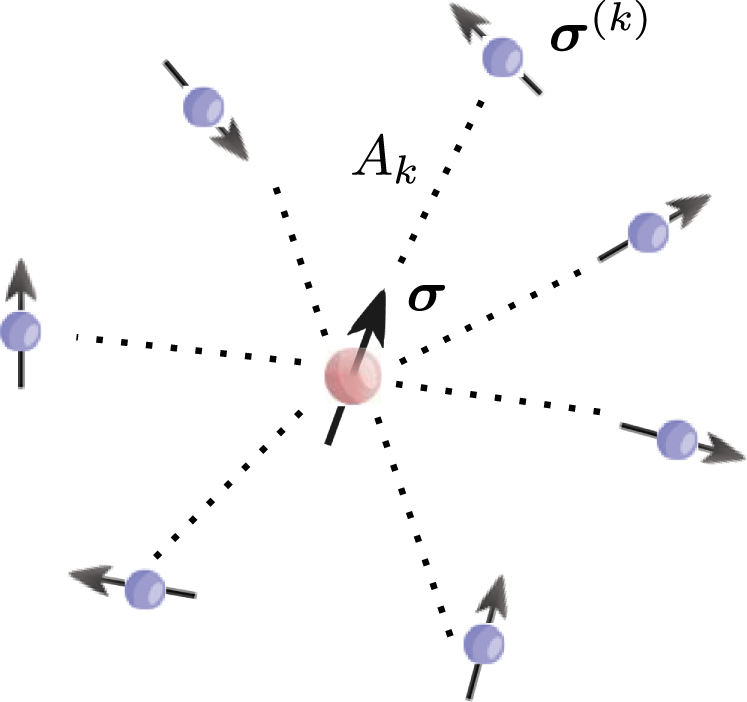
\includegraphics[width = 0.35\textwidth]{Abbildungen/CSM_Schema.jpg}
    \caption{Schematischer Aufbau des Central-Spin-Modells mit dem Elektronenspins (Rot) und den in direkter Umgebung liegenden 
    Kernspins (Blau) und einer Kopplungskonstante $A_k$}
    \label{fig:CSM}
\end{wrapfigure}
%CSM: https://iopscience.iop.org/article/10.1088/1367-2630/16/6/065023
Im folgenden wir das \textbf{Central Spin Model} zur Beschreibung der Spindynamik des Quantenpunktes verwendet. Dabei werden 
zu dem vorherigen Hamiltonian, die legiglich die Interaktionen des Elektrones mit mit einem externem Magnetfeld $\vec{B}$ berücksichtigt, 
fließen die Interaktionen der umliegenden Kernspins $\hat{\vec{I}}_k$ mit ein, d.h. die Wechselwirkung der Kernspins mit dem externen 
Magnetfeld und dem Elektronen-Spin über eine Heisenbergkopplung. Die Wechselwirkungen, der einzelnen Kernspins untereinander wird 
vernachlässigt.

\begin{align}
    \hat{H}_{CSM} &= \gamma_e \vec{B}\hat{\vec{S}} +  \sum_{k=1}^{N}\gamma_k\vec{B}\hat{\vec{I}}_k + \sum_{k=1}^{N}\alpha \hat{\vec{S}}\hat{\vec{I}}_k
\end{align}




\noindent Durch die Hinzunahme nur eines zusätzlich Kernspinors $\hat{\vec{I}}$ erhalten wir den einfachsten Fall des Central 
Spin Models, der Hamiltonian vereinfacht sich somit zu:

\begin{align}
    \hat{H} &= \underbrace{\gamma_e \vec{B}\hat{\vec{S}}}_{\hat{H}_1} + \underbrace{\gamma_k \vec{B}\hat{\vec{I}}}_{\hat{H}_2} + \underbrace{\alpha \hat{\vec{S}}\hat{\vec{I}}}_{\hat{H}_3}\\
\end{align}
mit $\gamma_e=\mu_B\thinspace g_e$ und  $\gamma_k=\mu_k\thinspace g_k$, wobei die Kopplung $\gamma_k$ zum Magnetfeld B deutlich 
schwächer als die des Elektrons $\gamma_e$ ist. Bei $\alpha$ handelt es sich um die Kopplungskonstante beider Spins.





%%%%%%% Klassischer Ansatz





\subsection{klassischer Ansatz}
\noindent Im ersten Schritt wird der klassische nicht-normierte Produktansatz $\ket{\Psi} = \ket{\Psi(\mu_1, \mu_2)}$: 
\begin{align}
    \ket{\Psi} &= e^{\mu_1 S_{1}^{-}}e^{\mu_2 S_{2}^{-}}\ket{\uparrow,\uparrow}\\
                &= \ket{\uparrow \uparrow} +\mu_1\ket{\downarrow \uparrow} + \mu_2\ket{\uparrow \downarrow} + \mu_1\mu_2\ket{\downarrow\downarrow}\\
                &= \underbrace{\left(\ket{\uparrow}_1 + \mu_1\ket{\downarrow}_1\right)}_{\ket{\Psi_1}}\underbrace{\left(\ket{\uparrow}_2 + \mu_2\ket{\downarrow}_2\right)}_{\ket{\Psi_2}}  \\
\end{align}





Damit ergibt sich für den modifizierten Hamiltonian: 

\begin{align}
    \mathcal{H} &= \frac{\bra{\Psi}\hat{H}_1\ket{\Psi}+ \bra{\Psi}\hat{H}_2\ket{\Psi} +\bra{\Psi}\hat{H}_3\ket{\Psi}}{\N}\\
\end{align}

Mit

\begin{align}
   \bra{\Psi}\hat{H_1}\ket{\Psi} &= \frac{\gamma_e}{2}(1+\mu_2\muk_2)\left(B_x(1-\mu_1^2) + iB_y(1+\mu_1^2) - 2\mu_1 B_z\right)\\
   \bra{\Psi}\hat{H_2}\ket{\Psi} &= \frac{\gamma_k}{2}(1+\mu_1\muk_1)\left(B_x(1-\mu_2^2) + iB_y(1+\mu_2^2) - 2\mu_2 B_z\right)\\
   \bra{\Psi}\hat{H}_3\ket{\Psi} &= \frac{\alpha}{4}\left[( \mu_1 + \muk_1)( \mu_2 + \muk_2) - (\mu_1-\muk_1)(\mu_2 - \muk_2) + (1-\mu_1\muk_1)(1-\mu_2\muk_2)\right]
\end{align}  


Und wir erhalten die partiellen Ableitungen:
\begin{align}
    \partial_{\muk_1}\mathcal{H} &= \underbrace{\frac{\gamma_1}{2(1+\mu_1\muk_1)^2}[B_x(1-\mu_1^2) + iB_y(1+\mu_1^2) - B_z\mu_1]}_{= \partial_{\muk_1} \frac{\bra{\Psi}\hat{H}_1 + \hat{H}_2\ket{\Psi}}{\N}} \\
    &+ \underbrace{\frac{\alpha}{2}\frac{(\mu_2 -\mu_1)(1+\mu_1\muk_2)}{(1+\mu_1\muk_1)^2(1+\mu_2\muk_2)}}_{= \partial_{\muk_1} \frac{\bra{\Psi}\hat{H}_3\ket{\Psi}}{\N}}\\
    \partial_{\muk_2}\mathcal{H} &= \underbrace{\frac{\gamma_2}{2(1+\mu_2\muk_2)^2}[B_x(1-\mu_2^2) + iB_y(1+\mu_2^2) - B_z\mu_2]}_{= \partial_{\muk_2} \frac{\bra{\Psi}\hat{H}_1 + \hat{H}_2\ket{\Psi}}{\N}} \\
    &+ \underbrace{\frac{\alpha}{2}\frac{(\mu_1 -\mu_2)(1+\mu_2\muk_1)}{(1+\mu_1\muk_1)(1+\mu_2\muk_2)^2}}_{= \partial_{\muk_2} \frac{\bra{\Psi}\hat{H}_3\ket{\Psi}}{\N}}
\end{align}

Um nun die DGL aufzustellen, fehlt nur noch die Berechnung der modifizierten Gram-Matrix, die diesmal zweidimensional ist. 
Wir erhalten nach einer längeren Rechnung:

\begin{align}
    G &=
    \begin{pmatrix}
        (1+\mu_1\muk_1)^2 & 0 \\
        0 &(1+\mu_2\muk_2)^2
    \end{pmatrix} \\
    G^{-1} &=
    \begin{pmatrix}
        \frac{1}{(1+\mu_1\muk_1)^2} & 0 \\
        0 &\frac{1}{(1+\mu_2\muk_2)^2}
    \end{pmatrix}
\end{align}

\noindent Nun können die Bewegungsgleichungen aufgestellt werden:
\begin{align}
    i\dot{\mu_1} &= \sum_{j}\left(G_{1j}\right)^{-1}\thinspace \partial_{\overline{\mu_j}}\mathcal{H}  \\
    &=\underbrace{\frac{\gamma_1}{2}B_x(1-\mu_1^2) + \frac{i\gamma_1}{2}B_y(1+\mu_1^2) -\mu_1 \gamma_1 B_z}_{\text{Ein-Spin-Präzession im } \vec{B}} +\underbrace{\frac{\alpha}{2} \frac{(\mu_2-\mu_1)(1+\mu_1\muk_2)}{1+\mu_2\muk_2}}_{\text{Ein-Spin-Präzession um } \frac{\bra{\Psi}\hat{\vec{I}}\ket{\Psi}}{\N}  }    
\end{align}
und analoger Weise 
\begin{align}
    i\dot{\mu_2} &= \underbrace{\frac{\gamma_2}{2}B_x(1-\mu_2^2) + \frac{i\gamma_2}{2}B_y(1+\mu_2^2) -\mu_2 \gamma_2 B_z}_{\text{Ein-Spin-Präzession im } \vec{B}} +\underbrace{\frac{\alpha}{2} \frac{(\mu_1-\mu_2)(1+\mu_2\muk_1)}{1+\mu_1\muk_1}}_{\text{Ein-Spin-Präzession um } \frac{\bra{\Psi}\hat{\vec{S}}\ket{\Psi}}{\N}  }
\end{align}

\noindent Aufgrund der Linearität der DGL ist die Lösung der ersten DGL aus dem Ein-Spin-Fall zu entlesen. Nun fehlt es noch zu beweisen, 
dass der letztere Summand die Präzession um den Spin-Erwartungswert des jeweilig anderen Spins.

\begin{align}
    \frac{\alpha}{2} \frac{(\mu_2-\mu_1)(1+\mu_1\muk_2)}{1+\mu_2\muk_2} &= 
     \frac{\alpha}{2}\left[\underbrace{\frac{1}{2}\frac{\mu_2 + \muk_2}{1+\mu_2\muk_2}}_{\frac{\bra{\Psi}\hat{I_x}\ket{\Psi}}{\N}}(1-\mu_1^2) + i \underbrace{\frac{i}{2}\frac{\muk_2 -\mu_2}{1+\mu_2\muk_2}}_{\frac{\bra{\Psi}\hat{I_y}\ket{\Psi}}{\N}}(1+\mu_1^2) - 2\mu_1\underbrace{\frac{1}{2}\frac{1-\mu_2\muk_2}{1+\mu_2\muk_2}}_{\frac{\bra{\Psi}\hat{I_z}\ket{\Psi}}{\N}} \right]
\end{align}
Hier lässt sich erkennen, dass die $\frac{\bra{\Psi}\hat{I_i}\ket{\Psi}}{\N}$ die Rolle des Magnetfeldes $\vec{B}$ im Ein-Spin-Lösung 
übernehmen. Wir erhalten dann aus Symmetriegründen:

\begin{align}
    \frac{d}{dt}\left[\frac{\bra{\Psi}\hat{\vec{S}}\ket{\Psi}}{\N}\right] &= \left(\gamma_1\vec{B} + \alpha \frac{\bra{\Psi}\hat{\vec{I}}\ket{\Psi}}{\N}\right)\cross\frac{\bra{\Psi}\hat{\vec{S}}\ket{\Psi}}{\N}\\
    \frac{d}{dt}\left[\frac{\bra{\Psi}\hat{\vec{I}}\ket{\Psi}}{\N}\right] &= \left(\gamma_2\vec{B} + \alpha \frac{\bra{\Psi}\hat{\vec{S}}\ket{\Psi}}{\N}\right)\cross\frac{\bra{\Psi}\hat{\vec{I}}\ket{\Psi}}{\N}
\end{align}
\noindent dabei ist zu bemerken, dass $\gamma_2$ deutlich kleiner als $\gamma_1$ ist, und die Heisenbergkopplung stark dominiert.\\
Wir erkennen, dass mit diesem Ansatz wie zu erwarten eine klassische Lösung erhalten, wo zwei Spin um einander präzedieren. Dabei 
taucht quantenmechanische Verschränkung nicht auf, da beide Spin-Längen konstant bleiben zu jedem beliebigen Startzeitpunkt.








%%%%%%%%%%%%% Quantenkorrektur













\subsection{modifizierter Ansatz: Quantenkorrektur}

\noindent Wir nehmen ohne Beschränkung der Allgemeinheit an, dass das Magnetfeld $\vec{B}$ in z-Richtung ausgerichtet ist. Somit vereinfacht sich die der Hamiltonian:
\begin{align}
    \hat{H} &= \gamma_e \vec{B}_z\hat{\vec{S}}_z +  \gamma_k\vec{B}_z\hat{\vec{I}}_z + \alpha \hat{\vec{S}}\hat{\vec{I}}
\end{align}


\noindent Um eine genauere Lösung zu erhalten, führen wir einen weiteren Korrekurparameter $\mu_{12}$ ein, wodurch ein größerer Unterraum des zwei 1/2-Spin-Hilbertraumes aufgespannt wird, mit der Hoffnung im Gegensatz zum klassischen Ansatz die Verschränkung zu berücksichtigen:


\begin{align}
    \ket{\Psi(\mu_1,\mu_2,\mu_{12})} &= e^{\mu_1 S_1^-}e^{\mu_2 S_2^-}e^{\mu_{12} S_1^-S_2^-}\ket{\uparrow,\uparrow}\\
                                    &= \ket{\uparrow \uparrow} +\mu_1\ket{\downarrow \uparrow} + \mu_2\ket{\uparrow \downarrow} + (\mu_1\mu_2 + \mu_{12})\ket{\downarrow \downarrow}
\end{align}
Mit diesem Ansatz erhalten wir nach längerer Rechnung den modifizierten Hamiltonian:

\begin{align}
    \mathcal{H} &= \frac{\bra{\Psi}\hat{H}_1\ket{\Psi} +\bra{\Psi}\hat{H}_2\ket{\Psi} + \bra{\Psi}\hat{H}_3\ket{\Psi}}{\N}
\end{align}
mit 
\begin{align*}
    \bra{\Psi}\hat{H}_1\ket{\Psi} &=  \frac{\gamma_1 B_z}{2}\left[ 1- \mu_1\muk_1 + \mu_2\muk_2 - (\mu_1 \mu_2 + \mu_{12})(\overline{\mu_1\mu_2} + \muk_{12})\right] \\
    %
    \bra{\Psi}\hat{H}_2\ket{\Psi} &=  \frac{\gamma_1 B_z}{2}\left[ 1- \mu_2\muk_2 + \mu_1\muk_1 - (\mu_1 \mu_2 + \mu_{12})(\overline{\mu_1\mu_2} + \muk_{12})\right] \\
    %
    \bra{\Psi}\hat{H}_3\ket{\Psi} &= \frac{\alpha}{4}[2(\muk_1\mu_2 + \mu_1\muk_2) + 1 - \mu_1\muk_1 - \mu_2\muk_2 + (\mu_1 \mu_2 + \mu_{12})(\overline{\mu_1\mu_2} + \muk_{12})]
\end{align*}

\noindent Damit folgen für die partiellen Ableitungen nach den konjugierten Parameter

\begin{align*}
    \partial_{\muk_1} \mathcal{H} &= 
    -B\gamma_1 \frac{\mu_1(1+\mu_2\muk_2)^2 + \muk_2\mu_{12}}{\N^2}\\
    &+B\gamma_2 \frac{\muk_{12}(\mu_1\mu_2 + \mu_{12})}{\N^2}\\
    &+\frac{\alpha}{2}\frac{(\mu_2-\mu_1)(\mu_1\muk_2+1)(1+\mu_2\muk_2)+\muk_{12}(\mu_1\mu_2 + \mu_{12}) + \mu_{12}\muk_2}{\N^2}\\
    %
    \partial_{\muk_2} \mathcal{H} &= 
    +B\gamma_1 \frac{\muk_{12}(\mu_1\mu_2 + \mu_{12})}{\N^2}\\
    &-B\gamma_2 \frac{\mu_2(1+\mu_1\muk_1)^2 + \muk_1\mu_{12}}{\N^2}\\
    &+\frac{\alpha}{2}\frac{(\mu_1-\mu_2)(\mu_2\muk_1+1)(1+\mu_1\muk_1)+\muk_{12}(\mu_1\mu_2 + \mu_{12}) + \mu_{12}\muk_1}{\N^2}\\
    %
    \partial_{\muk_{12}} \mathcal{H} &= 
    -B\gamma_1\frac{(\mu_1\mu_2+\mu_{12})(1+\mu_2\muk_2)}{\N^2}\\
    &-B\gamma_2\frac{(\mu_1\mu_2+\mu_{12})(1+\mu_1\muk_1)}{\N^2}\\
    &+\frac{\alpha}{2}\frac{(\muk_1-\muk_2)(\mu_1-\mu_2)(\mu_1\mu_2+\mu_{12}}{\N^2}
\end{align*}

\noindent Und für die Gram-Matrix erhalten wir:
\begin{align}
    G &=
    \begin{pmatrix}
        (1+\mu_1\muk_1)^2 + \mu_{12}\muk_{12} & -\mu_1^2\muk_{12} - \muk_2^2\mu_{12} &  \mu_2(1+\mu_2\muk_2)-\muk_1\mu_{12}\\
        -\mu_2^2\muk_{12} - \muk_1^2\mu_{12} &(1+\mu_2\muk_2)^2 + \mu_{12}\muk_{12} & \mu_1(1+\mu_1\muk_1)-\muk_2\mu_{12}\\
        \muk_2(1+\mu_2\muk_2)-\mu_1\muk_{12} & \muk_1(1+\mu_1\muk_1)-\mu_2\muk_{12} & 1 + \mu_1\muk_1 + \mu_2\muk_2
    \end{pmatrix}\frac{1}{\N^2} \\
\end{align}

Somit lassen sich die Bewegungsgleichungen der Parameter explizit aufschreiben:

\begin{align}
    i\dot{\mu}_1 &= G_{1,1}^{-1}\thinspace \partial_{\muk_1}\mathcal{H} + G_{1,2}^{-1}\thinspace\partial_{\muk_2}\mathcal{H} + G_{1,3}^{-1}\thinspace\partial_{\muk_3}\mathcal{H} \\
    i\dot{\mu}_2 &= G_{2,1}^{-1}\thinspace\partial_{\muk_1}\mathcal{H} + G_{3,2}^{-1\thinspace}\partial_{\muk_2}\mathcal{H} + G_{2,3}^{-1}\thinspace\partial_{\muk_3}\mathcal{H} \\
    i\dot{\mu}_{12} &= G_{3,1}^{-1}\thinspace\partial_{\muk_1}\mathcal{H} + G_{3,2}^{-1}\thinspace\partial_{\muk_2}\mathcal{H} + G_{3,3}^{-1}\thinspace\partial_{\muk_3}\mathcal{H} 
\end{align}



\subsection{quantenmechanischen Lösung}
Für die exakte quantenmechanische Lösung, wird der Hamiltonian diagonalisiert über die Basis:

\begin{align}
    \ket{1} &= \ket{\uparrow\uparrow}   \\
    \ket{2} &= \ket{\downarrow\downarrow} \\
    \ket{3} &= \frac{1}{\sqrt{2}N_1}\left[(\epsilon_1+1)\ket{\uparrow\downarrow} +(\epsilon_1-1)\ket{\downarrow\uparrow} \right]\\
    \ket{4} &= \frac{1}{\sqrt{2}N_2}\left[(\epsilon_2+1)\ket{\uparrow\downarrow} +(\epsilon_2-1)\ket{\downarrow\uparrow} \right]
\end{align}
mit $\epsilon_{1,2} = \frac{\alpha \pm \sqrt{B^2(\gamma_1-\gamma_2)^2+\alpha^2} }{B(\gamma_1-\gamma_2} $ und $N_{i} = \sqrt{\epsilon_i^2 + 1}$. Die dazugehörigen Eigenenergien lauten:
\begin{align}
    E_1 &= B(\gamma_1+\gamma_2) + \frac{\alpha}{4}\\
    E_2 &= -B(\gamma_1+\gamma_2) + \frac{\alpha}{4}\\
    E_3 &= -\frac{\alpha}{4} + \frac{\sqrt{\alpha^2 + B^2(\gamma_1-\gamma_2)^2}}{2}\\
    E_4 &= -\frac{\alpha}{4} - \frac{\sqrt{\alpha^2 + B^2(\gamma_1-\gamma_2)^2}}{2}\\
\end{align}
\noindent Über den Zeitentwicklungsoperator und einem beliebigen Startzustand $\ket{\Psi_0}$, lässt sich die Spindynamik hinschreiben als:

\begin{align}
    \bra{\Psi}\hat{S}_i\ket{\Psi} &= \sum_{i,j}e^{i(E_i-E_j)t}\bra{i}\hat{S}_i\ket{j}\bra{j}\ket{\Psi_0}\bra{\Psi_0}\ket{i}
\end{align}
    




\end{document}
